\documentclass{article}
\usepackage[utf8]{inputenc}
\usepackage{polski}
\usepackage{listings}
\usepackage{hyperref}
\usepackage{chngpage}
\usepackage{natbib}
\usepackage{graphicx}
\usepackage{url}

\title{\textbf{\huge{Urządzenia peryferyjne}} \\
        Czytnik kart chipowych}
\author{225942 Justyna Skalska \\
        226126 Grzegorz Kopacz}
\date{środa, 14\textsuperscript{15}-17\textsuperscript{15} TN\\[10pt]
    \today}

\begin{document}

\maketitle
\section{Opis zadania}
Podczas pierwszych zajęć laboratoryjnych nasza grupa miała zapoznać się z zasadą działania czytnika kart chipowych oraz jak korzystać z komend APDU. Przy użyciu przykładowej aplikacji zamieszczonej w instrukcji musieliśmy dostać się do danych zapisanych na karcie i pobrać z niej kilka pierwszych SMSów. Po ich pobraniu należało je przekodować i odczytać zawartą w nich treść oraz numery telefonów, z których zostały wysłane. Kolejnym zadaniem było stworzenie własnego programu potrafiącego odczytać dane z karty chipowej, ale zabrakło nam czasu na jego wykonanie. 

\section{Wstęp}
Karta chipowa, inaczej karta elektroniczna lub mikroprocesorowa to nośnik danych w postaci karty wykonanej z plastiku z umieszczonym na niej, lub wewnątrz niej, jednym lub kilkoma układami scalonymi.\citep{wiki}
Dzięki mikroprocesorowi można zapisywać oraz odczytywać dane umieszczone w pamięci. Oprócz niego na karcie znajduje się także pamięć ROM, w której zapisany jest system operacyjny. Dzieli on pamięć na 3 obszary (obszar swobodnego odczytu, obszar poufny oraz obszar roboczy przechowujący dane).\bigskip\\ 
Systemy plików na karcie elektronicznej: 
\begin{itemize}
    \item MF (master file) – korzeń drzewa katalogów (adres: 3F00).
    \item DF (dedicated file) – odpowiednik katalogu w systemach operacyjnych komputerów.
    \item EF (elementary file) – pliki z danymi.
\end{itemize}
\begin{figure}[ht]
\centering
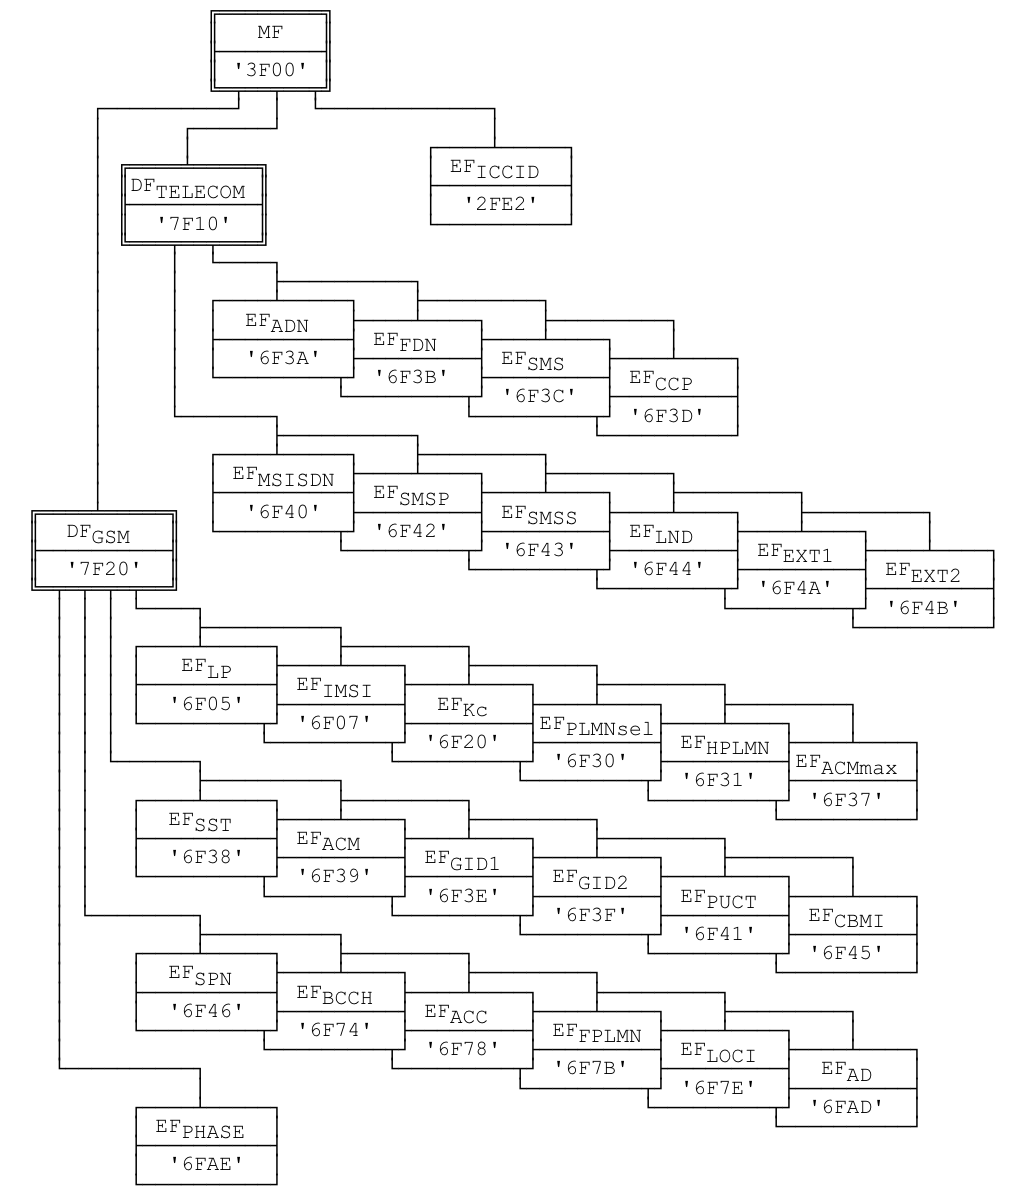
\includegraphics[width = 10cm]{directory_structure.png}
\caption{Identyfikatory plików i struktura katalogów GSM}\citep{gsmTechSpecs}
\label{fig:directory_structure}
\end{figure}
\bigskip 
Dzięki kodom APDU można dostać się do danych zawartych na karcie wykorzystując zamieszczoną wyżej strukturę katalogów. Istnieją dwie kategorie APDU, które różnią się od siebie formatem: rozkaz (command) oraz odpowiedź (response).
\newpage
\begin{table}[ht]
    \centering
    \begin{tabular}{|c|c|c|c|c|c|c|}
         \hline
         & CLA & INS & P1 & P2 & P3 & Data \\
         \hline
         Długość (bajty) & 1 & 1 & 1 & 1 & 1 & 256 \\
         \hline
    \end{tabular}
    \caption{Struktura rozkazu oraz maksymalna długość danych}
\end{table}
\begin{table}[ht]
    \centering
    \begin{tabular}{|c|c|c|c|}
        \hline
        & Data & SW1 & SW2 \\
        \hline
        Długość (bajty) & 256 & 1 & 1 \\
        \hline
    \end{tabular}
    \caption{Struktura odpowiedzi oraz maksymalna długość danych}
\end{table}

Znaczenie poszczególnych bajtów:
\begin{itemize}
    \item CLA - klasa instrukcji (w przypadku GSM jest to A0).
    \item INS - kod instrukcji do wykonania.
    \item P1/P2 - parametry rozkazu.
    \item P3 - długość danych rozkazu.
    \item Data - dane rozkazu lub odpowiedzi.
    \item SW1/SW2 - kod statusu odpowiedzi (rozkaz udany lub nieudany).
\end{itemize}

\section{Zadanie}
Zadanie polegało na odczytaniu SMSów zapisanych w pamięci karty elektronicznej. Skorzystaliśmy z podanych komend (S - dane wysłane, R - dane otrzymane):
\begin{enumerate}
\item A4 00 00 02 3F00 - wybranie głównego katalogu (MF - master file).
\item A4 00 00 02 7F10 - wybranie katalogu zawierającego funkcje usług telekomunikacyjnych (DF - dedicated file).
\item A4 00 00 02 6F3C - wybranie pliku z SMSami (EF - elementary file).
\item C0 00 00 0F - pobranie odpowiedzi o długości 0F.
\item B2 00 02 B0 - odczytanie wybranego rekordu (02 - tryb, w którym wskaźnik jest inkrementowany przed odczytem. Jeśli w wybranym EF nie odczytano jeszcze żadnego rekordu funkcja odczyta pierwszy rekord i ustawi na nim wskaźnik).
\item B2 01 02 B0 - odczytanie następnego rekordu.
\item B2 02 02 B0 - odczytanie następnego rekordu.
\end{enumerate}
\begin{table}[ht]
    \centering
    \begin{tabular}{|c|c|c|c|c|c|}
        \hline
        COMMAND & INS & P1 & P2 & P3 & S/R \\
        \hline
        SELECT & A4 & 00 & 00 & 02 & S/R \\
        READ RECORD & B2 & nr rekordu & tryb & długość & R \\
        GET RESPONSE & C0 & 00 & 00 & długość & R \\
        \hline
    \end{tabular}
    \caption{Kodowanie komend}
\end{table}
\newpage
\begin{table}[ht]
    \begin{adjustwidth}{-1in}{-1in}
    \centering
    \begin{tabular}{|c|c|c|c|}
        \hline
        SMS & Odpowiedź & Treść & Nadawca \\
        \hline
        1 & 0707918406921511F11100038111F10000000631D92C269B01 & 123123 & 111 \\
        2 & 0707918406921511F11100038133F300000006F7FBFD7EBF03 & wwwwww & 333 \\
        3 & 0707918406921511F111000881433224430000000964F3996C3E93CD67 & dfgdfgdfg & 34234234 \\
        \hline
    \end{tabular}
    \end{adjustwidth}
    \caption{Odczytane SMSy}
\end{table}
Aby odkodować wiadomości posłużyliśmy się aplikacją na stronie: \url{https://www.diafaan.com/sms-tutorials/gsm-modem-tutorial/online-sms-pdu-decoder/}
\section{Wnioski}
\bibliographystyle{plain}
\bibliography{references}
\end{document}
